\documentclass{article}

\usepackage[russian,english]{babel}
\usepackage[T1]{fontenc}
\usepackage[utf8]{inputenc}
\usepackage{amsmath,amssymb}
\usepackage{mathtext}
\usepackage{graphicx}


\begin{document}

\selectlanguage{russian}

\tableofcontents
\pagebreak

\section{Введение}

В данной статье приводится описание программы, позволяющей моделировать систему идеальных жёстких сфер вблизи идеальных стенок. Описывается модель жёстких сфер, модель идеальной стенки и модель используемых периодических граничных условий.

Описание, приведённое в данной статье, соответвует программе, написанной для моделирования исследуемой нами системы жёстких сфер, и может быть использовано для анализа алгоритма, реализованного в написанной программе.

Программа, реализующая описанный в этой статье алгоритм, написана на языке С++. Существует несколько версий программы, в которых реализация периодических граничных условий и некоторых функций может отличаться от описанного в этой статье алгоритма, в данной статье описывается только последний вариант реализации алгоритма, актуальный на данный момент, а так же приводится краткий обзор используемых ранее алгоритмов и периодических граничных условий с целью исторического обзора пути развития применяемых нами алгоритмов, а так же в целях объяснения причин, по которым мы выбрали имеено данные граничные условия и определённую реализацию некоторых алгоритмов (выбор используемых алгоритмов, в основном, продиктован их оптимальностью - предпочтение отдавалось алгоритмам, требующим наименьшего времени для получения точного решения).

В разработке физической модели моделируемой системы и алгоритма, описанного в данной статье и реализованного в программе на языке С++, принимали активное участие:

Вешнев Владимир Петрович

Гераськин Алексей ?

Нурлыгаянова Марина Николаевна

Нурлыгаянов Тимур Артурович

Данная статья и любая информация, описанная в ней, а так же исходный код программы, релизующий данный алгоритм, может быть использован, изменён или опубликован только с согласия всех описанных лиц.

\newpage
\section{Общее описание моделируемой системы}

\newpage
\section{Рассчёт столкновения идеальных жёстких сфер}

\subsection{Расчёт времени до соударения двух идеальных жёстких сфер}


\subsection{Расчёт новых скоростей идеальных жёстких сфер после соударения}
    \paragraph{}Рассмотрим общий случай соударения двух частиц, представляющих из себя идеальные жёсткие сферы:

\begin{center}
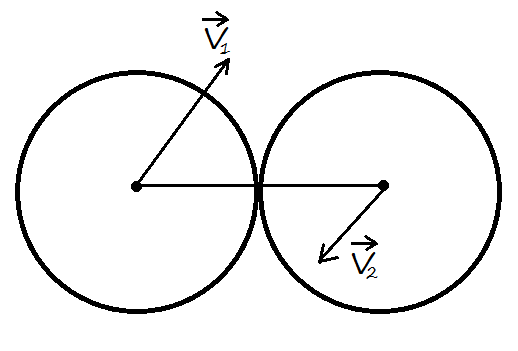
\includegraphics[scale=0.3]{collission_of_two_particles.png}
\end{center}

Здесь $ \vec{v}_1 $ - скорость первой частицы, $ \vec{v}_2 $ - скорость второй частицы.

Распишем скорость $ \vec{v}_1 $ как сумму $ \vec{v}_{1\perp} $ и $ \vec{v}_{1\parallel} $ и скорость $ \vec{v}_2 $ как сумму $ \vec{v}_{2\perp} $ и $ \vec{v}_{2\parallel} $, где $ \vec{v}_{1\perp} $ и $ \vec{v}_{2\perp} $ составляющие скоростей $ \vec{v}_1 $ и $ \vec{v}_2 $, перпендикулярные линии, соединяющей центры сталкивающихся частиц, $ \vec{v}_{1\parallel} $ и $ \vec{v}_{2\parallel} $ - составляющие скоростей $ \vec{v}_1 $ и $ \vec{v}_2 $, параллельные линии, соединяющей центры частиц.

При соударении этих частиц должен выполняться закон сохранения энергии и закон сохранения импульса. Закон сохранения импульса для рассматриваемой системы двух частиц в скалярном виде  может быть записан как

\begin{equation}\label{eq:rule_of_contant_impulse}
    \begin{cases}
        v_{1\perp} + v_{2\perp} = v'_{1\perp} + v'_{2\perp},
        \\
        v_{1\parallel} + v_{2\parallel} = v'_{1\parallel} + v'_{2\parallel},
    \end{cases}
\end{equation}
где $ v'_{1\perp} $, $ v'_{1\parallel} $, $ v'_{2\perp} $, $ v'_{2\parallel} $ - скорости частиц после соударения.

Запишем закон сохранения энергии для системы из двух сталкивающихся идеальных сфер:

\begin{equation}\label{eq:rule_of_contant_energy}
    \begin{cases}
        E_1 = v^2_{1\perp} + v^2_{1\parallel} + v^2_{2\perp} + v^2_{2\parallel},
        \\
        E_2 = v'^2_{1\perp} + v'^2_{1\parallel} + v'^2_{2\perp} + v'^2_{2\parallel},
        \\
        E_1 = E2,
    \end{cases}
\end{equation}
где $ E_1 $ - полная кинетическая энергия системы из двух частиц перед соударением, $ E_2 $ - полная кинетическая энергия системы из двух частиц после соударения. Потенциальная энергия частиц в рассматриваемой системе всегда равна нулю, т.к. в рассматриваемой системе не существует потенциальных полей дальнего действия.

Надо переделать вывод этого уравнения:
Идеальные жёсткие сферы соударяются абсолютно упруго и изменение скоростей частиц произойдёт только вдоль линии, соединяющей центры этих частиц. Исходя из этого предположения, мы можем записать:

\begin{equation}\label{eq:new_velocities_after_collission}
    \begin{cases}
        v_{1\perp} = v_{1\perp},
        \\
        v_{2\perp} = v_{2\perp},
        \\
        v'_{1\parallel} = v_{2\parallel},
        \\
        v'_{2\parallel} = v_{1\parallel},
    \end{cases}
\end{equation}

Запишем выражения для закона сохранения импульса (\ref{eq:rule_of_contant_impulse}) и закона сохранения энергии системы (\ref{eq:rule_of_contant_energy}) с учётом новых скоростей (\ref{eq:new_velocities_after_collission}), чтобы проверить соблюдение этих законов для случая, когда после соударения двух идеальных жёстких сфер их скорости меняются согласно (\ref{eq:new_velocities_after_collission}).

Выражение для закона сохранения импульса с учётом (\ref{eq:new_velocities_after_collission}) принимает вид:

\begin{equation}
    \begin{cases}
        v_{1\perp} + v_{2\perp} = v_{1\perp} + v_{2\perp},
        \\
        v_{1\parallel} + v_{2\parallel} = v_{1\parallel} + v_{2\parallel},
    \end{cases}
\end{equation}
где все слагаемые сокращаются, что означает выполнение закона сохранения момента импульса для данного случая.

Выражение для закона сохранения энергии системы двух частиц с учётом (\ref{eq:new_velocities_after_collission}) принимает вид:



\newpage
\section{Начальное состояние системы. Посев}

\subsection{Посев}

Для начала моделирования необходимо создать N жетких сфер в моделируемой системе таким образом, чтобы центры всех частиц находились в исследуемом объёме, частицы не проникали друг в друга, а так же чтобы начальный импульс системы и момент импульса системы по осям $ OX $, $ OY $ и $ OZ $ были равны нулю.

Процедура инициализации начальных параметров объёма, положений частиц и их скоростей называется "посев". В дальнейшем мы будем использовать этот термин для обозначения функции программы, которая позволяет произвести начальную инициализацию моделируемой системы.

Начальная плотность данной системы $ \eta_0 $ будет определяться задаваемым параметрами объёма исследуемой системы и количеством частиц в данном объёме (т.к. радиус идеальных жёстких сфер $R$ по умолчанию равен 1.0, мы полагаем его постоянным и одинаковым для всех частиц).

Изначально центры частиц размещаются в системе в "узлах" объёмо-центрированной кристаллической решётки, расстояние между частицами регулируется начальной плотностью системы, но при этом расстояние между двумя частицами не может быть меньше, чем два радиуса идеальных сфер (чтобы частицы не проникали друг в друга).

Расчёт начальных координат и скоростей идеальных сфер производится в несколько этапов, рассмотрим их более побробно:

1. Создаётся "кристалл" жёстких сфер с объёмо-центрированной кристаллической рещёткой, содержащий M частиц. Частицы в данном кристалле касаются друг друга и образуют прямоугольный параллепипед, рёбра которого по $ Y $ и $ Z $ равны между собой, при этом рёбра по $ X $ примерно в два раза больше рёбер по $ Y $ и $ Z $. Это продиктовано особенностями моделируемой системы, т.к. нам необходимо задавать длину системы L в четыре раза больше, чем размер системы по $ Y $ и $ Z $, чтобы иметь возможность исследовать свойства кристалла вблизи идеальной стенки, исключая при этом влияние второй, противоположной идеальной стенки, которая будет достаточно удалена от исследуемой части системы.

Один из углов данного параллепипеда будет совпадать с началом координат.

Расстояние между двумя одинаковыми слоями объёмо-центрированного кристалла в случае плотного соприкасания слоёв равно $ 2*\sqrt{2} $:

\begin{center}
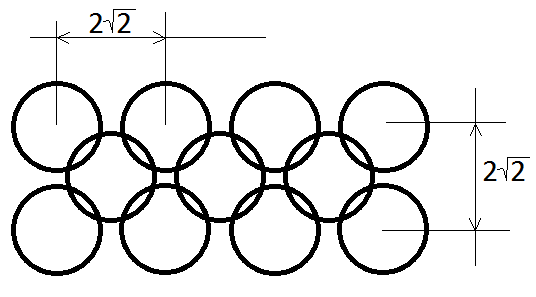
\includegraphics[scale=0.5]{distance_between_particles.png}
\end{center}

Координаты центра данного прямоугольного параллелепипеда можно рассчитать по формулам:

\begin{equation}\label{eq:r_scalar}
    \begin{cases}
        y = \displaystyle\frac{r_b * (NN - 1.0) + 2.0}{2.0},
        \\
        \\
        z = \displaystyle\frac{r_b * (NN - 1.0) + 2.0}{2.0},
        \\
        \\
        x = \displaystyle\frac{r_b * (2.0 * NN - 1.0) + 2.0}{2.0}.
    \end{cases}
\end{equation}
где $ r_b $ - это расстояние между одинаковыми слоями объёмо-центрированного кристалла, равное $ 2*\sqrt{2} $, NN - количество частиц в ребре куба по $ Y $ и $ Z $, это число задаётся при новом "посеве" частиц (см. главу "Описание управляющих команд программы").

2. Созданный кристалл копируется несколько раз так, чтобы увеличить кристалл вдвое по трём измерениям ($x$, $y$, $z$), таким образом, делается 7 копий созданного на шаге №1 кристалла, которые располагаются вплотную к первонаальному кристаллу так, чтобы частицы, находящиейся на границах параллепипедов, касались друг друга.

В результате получается кристалл жёстких сфер в форме прямоугольно параллепипеда, один угол которого совпадает с началом координат и одна сторона которого в два раза больше двух других сторон.

3. Для частиц, находящихся в кристалле, созданном на шаге №1, случайным образом задаются скорости $ v_x $, $ v_y $ и $ v_z $, при этом скорости остальных частиц в системе задаются так, чтобы суммарный импульс и момент импульса системы были равны нулю.

4. Основываясь на задаваемой плотности системы рассчитываются параметры моделируемого объёма $ A $ и $ L $, а так же коэффициент расширения $ \beta $ (мы рассмотрим подробнее вывод коэффициента расширения системы чуть ниже), на который умножаются все координаты частиц, благодаря чему объёмо-центрированный кристалл жёстких сфер расширяется до размеров моделируемой системы и частицы перестают касаться друг друга. При этом суммарный испульс и момент импульса системы остаются равными нулю, т.к. импульсы одних частиц уравновешены испульсами других частиц, расположенных симметрично относительно центра моделируемой системы.

5. Все частицы копируются ещё раз и их координаты изменяются параллельным переносом вдоль оси $ OX $ так, чтобы в результате частицы заполнили весь объём системы, заданный из рассчёта $ L = 4*A $. Скорости частиц не изменяются, поэтому общий импульс и момент импульса системы при этом так же не изменяются. Таким образом размер системы вдоль оси $ OX $ получается в четыре раза больше размера системы вдоль осей $ OY$ и $ OZ $, центры идеальных сфер распределены по всему объёму моделируемой системы так, чтобы частицы не проникали друг в друга и суммарный импульс системы и момент импульса системы были равны нулю.

После проведения "посева" состояние системы сохраняется во временный файл и загружается из него. Во время загрузки сохранённого состояния системы мы рассчитываем ближайшие события для каждой частицы и начинаем рассчёт динамики системы. Более подробно это описано в главе "Сохранение и загрузка состояния системы".

\subsection{Расчёт коэффециента расширения системы $ \beta $ }
Рассмотрим подробнее вывод коэффициента расширения системы $ \beta $.


\newpage
\section{Граничные условия}

В рассматриваемой нами системе существуют два типа граничных условий:

1. Идеальная стенка

2. Периодические граничные условия

В случае идеальной стенки идеальная жёсткая сфера соударяется с идеальной стенкой по закону абсолютно упругого удара, при этом энергия частицы не изменяется, изменяется лишь проекция скорости частицы на ось $ OX $:

\begin{equation}
v'_x = -v_x,
\end{equation}
где $ v_x $ - проекция скорости частицы на ось $ OX $ до соударения с идеальной стенкой, $ v'_x $ - проекция скорости частицы на ось $ OX $ после соударения с идеальной стенкой.

Условия соударения с идеальными стенками в рассматриваемой системе можно записать так:

\begin{equation}\label{eq:condition_of_collision_with_ideal_wall}
    \begin{cases}
        x = R, v_x < 0.0
        \\
        or
        \\
        x = L - R, v_x > 0.0,
    \end{cases}
\end{equation}
где $ x $ - это значение координаты частицы вдоль оси $ OX $, $ v_x $ - значение проекции скорости частицы на ось $ OX $, $ R $ - радиус идеальных сфер, равный 1.0, $ L $ - расстояние между двумя идеальными стенками. Частицы не могут находиться на расстоянии менее R от идеальной стенки и координаты всех частиц в системе в любой момент времени удовлетворяют следующим правилам:

\begin{equation}\label{eq:particles_and_ideal_wall}
    \begin{cases}
        x >= R
        \\
        x <= L - R.
    \end{cases}
\end{equation}

Периодические граничные условия не дают частицам беспрепятственно покидать выделенный объём, позволяя тем самым моделировать бесконечную систему частиц, рассчитывая динамику системы, содержащую только небольшое количество частиц.

Условия, которые накладываются на частицы, находящиеся в моделируемой системе:

1. Центр каждой частицы всегда находится в системе или на её границе. Положения центров каждой частицы в системе в любой момент времени удовлетворяют следующей системе уравнений:

\begin{equation}
    \begin{cases}
        x >= R,
        \\
        x <= L - R,
        \\
        0 <= y <= A,
        \\
        0 <= z <= A,
    \end{cases}
\end{equation}
где $ x $, $ y $ и $ z $ - координаты частицы в трехмерной системее координат, R - радиус частицы, представляющей из себя идеальную жесткую сферу, L - расстояние между двумя идеальными стенками и A - это расстояние между двумя противоположными плоскостями, представляющими периодические границы.

2. Частицы могут пересекать границы системы, заданные уравнениями:

\begin{equation}
y = 0
\end{equation}
\begin{equation}
y = A
\end{equation}
\begin{equation}
z = 0
\end{equation}
\begin{equation}
z = A
\end{equation}

И не могут пересекать границы, заданные уравнением:

\begin{equation}
x = 0
\end{equation}
\begin{equation}
x = L
\end{equation}

т.к. эти границы являются идеальными стенками. 

При пересечении границы в момент пересечения одной из периодических границ системы центром частицы на одной из других периодических границ создаётся частица с энергией, равной энергии данной частицы и движущаяся согласно тому же уравнению движения, что и исходная частица. Исходная частица, пересекающая границу системы, при этом удаляется.

3. Если для координат центра частицы выполняется одно из следующих условий:

\begin{equation}
0 <= y <= 1
\end{equation}
\begin{equation}
A - 1 <= y <= A
\end{equation}
\begin{equation}
0 <= z <= 1
\end{equation}
\begin{equation}
A - 1 <= z <= A
\end{equation}
то существует один "образ" данной частицы, который движется согласно тому же уравнению движения, что и исходная частица. При пересечении центром частицы одной из границ системы "образ" становится обычной частицей, а сама частица уничтожается. При этом энергия частицы не изменяется, меняются лишь координаты центра частицы.

4. Центр "образа" всегда находится вне системы, что позволяет не учитывать "образ" как отдельную частицу. Любой частице в системе может соответвовать либо ни одного "образа", либо только один "образ".

5. При столкновении частицы или ее "образа" с другой частицей, "образом" другой частицей или идеальной стенкой скорость частицы изменяется, как и её уравнение движения. При этом "образ", соответвующий этой частице, уничтожается (если он существовал) и создаётся новый "образ" (если это необходимо - см. пункт №3), который будет двигаться согласно новому уравнению движения.

6. "Образ" может иметь скорость, отличную от скорости самой частицы, при этом он обязательно должен перемещаться согласно тому же уравнению движения, что и исходная частица (по той же линии скорости или по линии скорости, полученной параллельным переносом по OX, что будет рассмотренно отдельно). При столкновении "образа" с другой частицей или "образом" другой частицы учитывается скорость исходной частицы, а не её "образа" (при рассчёте новых скоростей), что позволяет сохранять общую энергию системы постоянной.

7. При создании "образа" некоторой частицы позиция его центра выбирается так, чтобы он находился на линии скорости исходной частицы, в точке, из которой он достигнет одной из периодических границ системы в то же самое время, когда центр исходной частицы будет находиться в плоскости пересекаемой ею границы.

Рассмотрим подробнее вычисление координат центра создаваемого "образа". Уравнение движения центра сферы по прямолинейной траектории с постоянной скоростью в вектоном виде можно записать так:

\begin{equation}
\vec{r} = \vec{r}_0 + \vec{v}*t
\end{equation}

где $ \vec{r} $ - радиус вектор нового положения центра частицы, $ \vec{r}_0 $ - радиус вектор начального положения центра частицы, $ \vec{v} $ - скорость частицы и $ t $ - время движения.

Распишем это выражение в проекциях на оси координат:

\begin{equation}\label{eq:r_scalar}
    \begin{cases}
        r_x = r_{0x} + v_x * t,
        \\
        r_y = r_{0y} + v_y * t,
        \\
        r_z = r_{0z} + v_z * t.
    \end{cases}
\end{equation}

из этой системы уравнений получаем:

\begin{equation}\label{eq:t_simple}
    \begin{cases}
        t = \displaystyle\frac{r_x - r_{0x}}{v_x},
        \\
        t = \displaystyle\frac{r_y - r_{0y}}{v_y},
        \\
        t = \displaystyle\frac{r_z - r_{0z}}{v_z}.
    \end{cases}
\end{equation}

Полученная система уравнений (\ref{eq:t_simple}) позволяет рассчитывать время, требующееся для перемещения центра частицы из одной позиции в другую.

Когда центр частицы находится на границе системы, прямая, описывающая уравнение её движения, пересекает плоскость, которой описана эта граница. Рассчитав времена, которые потребуются частице для того, чтобы её центр оказался в плоскости каждой границы, мы можем вычислить границу, на которой центр выбранной частицы окажется быстрее всего. Для этого необходимо решить четыре системы уравнений (одна система уравнений для каждой периодической границы):

\begin{equation}
    \begin{cases}
        y = 0,
        \\
        t = \displaystyle\frac{r_y - r_{0y}}{v_y}.
    \end{cases}
\end{equation}

\begin{equation}
    \begin{cases}
        y = A,
        \\
        t = \displaystyle\frac{r_y - r_{0y}}{v_y}.
    \end{cases}
\end{equation}

\begin{equation}
    \begin{cases}
        z = 0,
        \\
        t = \displaystyle\frac{r_z - r_{0z}}{v_z}.
    \end{cases}
\end{equation}

\begin{equation}
    \begin{cases}
        z = A,
        \\
        t = \displaystyle\frac{r_z - r_{0z}}{v_z}.
    \end{cases}
\end{equation}

полагая при решении этих систем уравнений $ r_y = y $ и $ r_z = z $, мы получим 4 решения для  $t$:

\begin{equation}\label{eq:t_end}
    \begin{cases}
        t_1 = \displaystyle\frac{0 - r_{0y}}{v_y},
        \\
        t_2 = \displaystyle\frac{A - r_{0y}}{v_y},
        \\
        t_3 = \displaystyle\frac{0 - r_{0z}}{v_z},
        \\
        t_4 = \displaystyle\frac{A - r_{0z}}{v_z}.
    \end{cases}
\end{equation}
где $ r_{0y} $, $ r_{0z} $ - проекции радиус вектора текущего положения частицы на оси $ OY $ и $ OZ $.

Необходимо найти $ t_{min} $, удовлетворяющее условиям:

\begin{equation}\label{eq:t_min}
    \begin{cases}
        t_{min} > 0,
        \\
        t_{min} <= t_1,
        \\
        t_{min} <= t_2,
        \\
        t_{min} <= t_3,
        \\
        t_{min} <= t_4,
    \end{cases}
\end{equation}
где $ t_{min} $ есть время, за которое частица достигнет близжайшей границы системы, если будет двигаться с текущей скоростью. В соответвии с условием №7 'образ', соответвующий данной частице, должен  за это же время достигнуть другой периодической границы системы.

Для того, чтобы вычислить координаты центра создаваемого "образа", возьмём новые значения $ v_x $, $ v_y $ и $ v_z $, равные:

\begin{equation}
    \begin{cases}
        v'_x = - v_x,
        \\
        v'_y = - v_y,
        \\
        v'_z = -v_z.
    \end{cases}
\end{equation}

и рассчитаем для них уравнения (\ref{eq:t_end}) и (\ref{eq:t_min}), подставив полученное в результате решения этих уравнений значение $ t'_{min} $  значения $ v'_x $, $ v'_y $ и $ v'_z $ в систему уравнений (\ref{eq:r_scalar}), получим:

\begin{equation}
    \begin{cases}
        r'_x = r_{0x} + v'_x * t'_{min},
        \\
        r'_y = r_{0y} + v'_y * t'_{min},
        \\
        r'_z = r_{0z} + v'_z * t'_{min}.
    \end{cases}
\end{equation}
где $ r'_x $, $ r'_y $ и $ r'_z $ есть значения новых координат центра частицы, которые она будет иметь после прохождения через периодическую границу.

Сложив $ t_{min} $ и $ t'_{min} $ и подставив получившееся значение $ t $ в систему уравнений (\ref{eq:r_scalar}) мы получим значения координат создаваемого образа, соответвующего данной частице:

\begin{equation}
    \begin{cases}
        r''_x = r_{0x} + v'_x * (t_{min} + t'_{min}),
        \\
        r''_y = r_{0y} + v'_y * (t_{min} + t'_{min}),
        \\
        r''_z = r_{0z} + v'_z * (t_{min} + t'_{min}).
    \end{cases}
\end{equation}
здесь $ r''_x $, $ r''_y $ и $ r''_z $ - координаты создаваемого образа, $ r_{0x} $, $ r_{0y} $ и $ r_{0z} $ - текущие координаты исходной частицы, для которой необходимо создать виртуальную частицу.

\newpage
\section{Динамика моделируемой системы. События}
\subsection{Изменение положения частиц в системе}

\subsection{Типы событий}

В рассматриваемой нами системе могут происходить следующие события:

1. Соударение частицы или её "образа" с идеальной стенкой.

2. Соударение частицы или её "образа" с другой частицей или "образом" другой частицы.

3. Создание "образа" для частицы, находящейся в области, близкой к периодическим граничным условиям.

4. Переход частицы из одной "ячейки" в другую.

5. Замена "образа" частицей - "перерождение" частицы при прохождении через периодические граничные условия.

6. Удаление "образа" частицы.

\newpage
\section{Собственные времёна частиц и глобальное время системы}

\subsection{Синхронизация частиц}

\subsection{Поиск ближайшего события для частицы}

\newpage
\section{Бинарное дерево как структура данных}
Бинарное (двоичное) дерево - структура данных, хорошо известная в информатике. Позволяет сохранять упорядоченные по ключу данные так, что операции добавления и удаления элементов из такой структуры данных  имеют алгоритмическую сложность $ \log_2{N} $, в то время как удаление произвольного элемента из упорядоченного списка имеет алгоритмическую сложность $ N $, а добавление нового элемента в упорядоченный список имеет алгоритмическую сложность $ N*\log_2{N} $ (поиск позиции и вставка элемента с перестановкой всех элементов "вправо").

\subsection{Бинарное дерево как структура данных}

\subsection{Добавление элемента в бинарное дерево}

\subsection{Удаление элемента из бинарного дерева}

\subsection{Сравнение алгоритмов на основе бинарного дерева и линейного массива}

\subsection{Бинарное дерево для сохранения информации о всех ближайших событиях в системе}


\newpage
\section{Сохранение и загрузка состояния системы}

\newpage
\section{Измерение относительной плотности}

\newpage
\section{Получение данных о структуре системы}
\subsection{Профиль плотности}
\subsection{Исследование структуры выделенного слоя частиц. Разрезы}

\newpage
\section{Изменение объёма системы}

\newpage
\section{Измерение давления}
Данная часть алгоритмов и программы ещё не реализовано, необходимо добавить описание того, как мы будем производить измерения данных и описать реализацию алгоритма в программе.

\newpage
\section{Измерение химического потенциала}
Данная часть алгоритмов и программы ещё не реализовано, необходимо добавить описание того, как мы будем производить измерения данных и описать реализацию алгоритма в программе.


\newpage
\section{Описание управляющих команд программы}

\newpage
\section{Глоссарий}

\end{document}